% BLAST Extension
%
% Basic description of the extension stage of the BLAST algorithm

\subsection{BLAST Extension}
\begin{frame}
  \frametitle{Extension}
  \begin{itemize}
    \item The best-scoring seeds are extended in each direction
    \item BLAST does not explore the complete search space, so a rule (heuristic) to stop extension is needed
    \item Two-stage process:
    \begin{itemize}
      \item Extend, keeping alignment score, and \emph{drop-off} score
      \item When drop-of score reaches a threshold $X$, trim alignment back to top score
    \end{itemize}
  \end{itemize}
  \begin{center}
    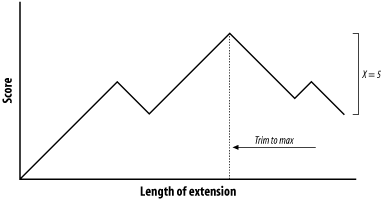
\includegraphics[width=0.5\textwidth]{images/extension} 
  \end{center}    
\end{frame}

\begin{frame}
  \frametitle{Example}
  \begin{itemize}
    \item<1-> Consider two sentences (match=+1, mismatch=-1)
    \begin{itemize}
      \item \texttt{The quick brown fox jumps over the lazy dog.}
      \item \texttt{The quiet brown cat purrs when she sees him.}
    \end{itemize}
    \item<2-> Extend to the right from the seed \texttt{T}
    \begin{itemize}
      \item \texttt{The quic}
      \item \texttt{The quie}
      \item \texttt{123 4565 <- score}
      \item \texttt{000 0001 <- drop-off score}        
    \end{itemize}
  \end{itemize}
\end{frame}

\begin{frame}
  \frametitle{Example}
  \begin{itemize}
    \item Consider two sentences (match=+1, mismatch=-1)
    \begin{itemize}
      \item \texttt{The quick brown fox jumps over the lazy dog.}
      \item \texttt{The quiet brown cat purrs when she sees him.}
    \end{itemize}
    \item Extend to drop-off threshold
    \begin{itemize}
      \item \texttt{The quick brown fox jump}
      \item \texttt{The quiet brown cat purr}
      \item \texttt{123 45654 56789 876 5654 <- score}
      \item \texttt{000 00012 10000 123 4345 <- drop-off score}        
    \end{itemize}
  \end{itemize}
\end{frame}

\begin{frame}
  \frametitle{Example}
  \begin{itemize}
    \item Consider two sentences (match=+1, mismatch=-1)
    \begin{itemize}
      \item \texttt{The quick brown fox jumps over the lazy dog.}
      \item \texttt{The quiet brown cat purrs when she sees him.}
    \end{itemize}
    \item Trim back from drop-off threshold to get optimal alignment
    \begin{itemize}
      \item \texttt{The quick brown}
      \item \texttt{The quiet brown}
      \item \texttt{123 45654 56789 <- score}
      \item \texttt{000 00012 10000 <- drop-off score}        
    \end{itemize}
  \end{itemize}
\end{frame}

\begin{frame}
  \frametitle{Notes on implementation}
  \begin{itemize}
%    \item This example represents ungapped BLAST; gapped BLAST is more similar to dynamic programming
    \item $X$ controls termination of alignment extension, but dependent on:
    \begin{itemize}
      \item substitution matrix
      \item gap opening and extension parameters
    \end{itemize}
  \end{itemize}
  \begin{center}
    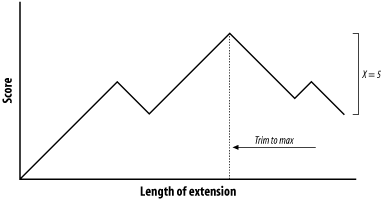
\includegraphics[width=0.5\textwidth]{images/extension} 
  \end{center}    
\end{frame}